\documentclass[12pt]{article}
\usepackage{amsmath,mathtools,amssymb,amsfonts, amsthm}
\usepackage{graphicx}
\begin{document}

\title{STAT 8004, Homework 1 REDO}
\author{Nooreen S. Dabbish}
\date{\today}

\maketitle

\textbf{Problem 1.} (30 points, 10 for each sub-problem)

Please use \LaTeX\ to input the following math equations.

a). 
\begin{align*}
f(y\mid\psi) &= \prod_{i=1}^{n} \rho_{ij}\\
             &= \prod_{i=1}^{n} \frac{\exp[u_{ij}(x_{i},z_{j})]}{\sum_{l=1}^{p}\exp[u_{ij}(x_{i},z_{l})]}
\end{align*}
\par b). 
\begin{align*}
\mathbf{V} &= \int_{0}^{1}\int_{0}^{\sqrt{1-x^2}} 2x^3 y \mathrm{d}y\mathrm{d}x\\
           &= \int_{0}^{1} x^3 y^2\bigg|_{y=0}^{y=\sqrt{1-x^2}} \mathrm{d}x.
\end{align*}

c). 
$$\boldsymbol{\begin{pmatrix}
\Omega' &\frac{1}{2}C'\\
C &0 \end{pmatrix}
\begin{pmatrix}
x \\ \lambda
\end{pmatrix}
=
\begin{pmatrix}
\omega \\ 0
\end{pmatrix}}$$

\vspace{3ex}

\textbf{Problem 2.} (10 points) Let $X = 0,\ 0.01,\ \ldots,\ 2$, and let $Y =
sin(X)$. Plot $Y$ vs $X$ in R. The $x$-axis should correspond to
the variable $X$ and the $y$-axis should correspond to the variable
$Y$. Please put the figure here, and caption it as ``A figure to show
relationship between $X$ and $Y$''. 

\begin{figure}
\centering
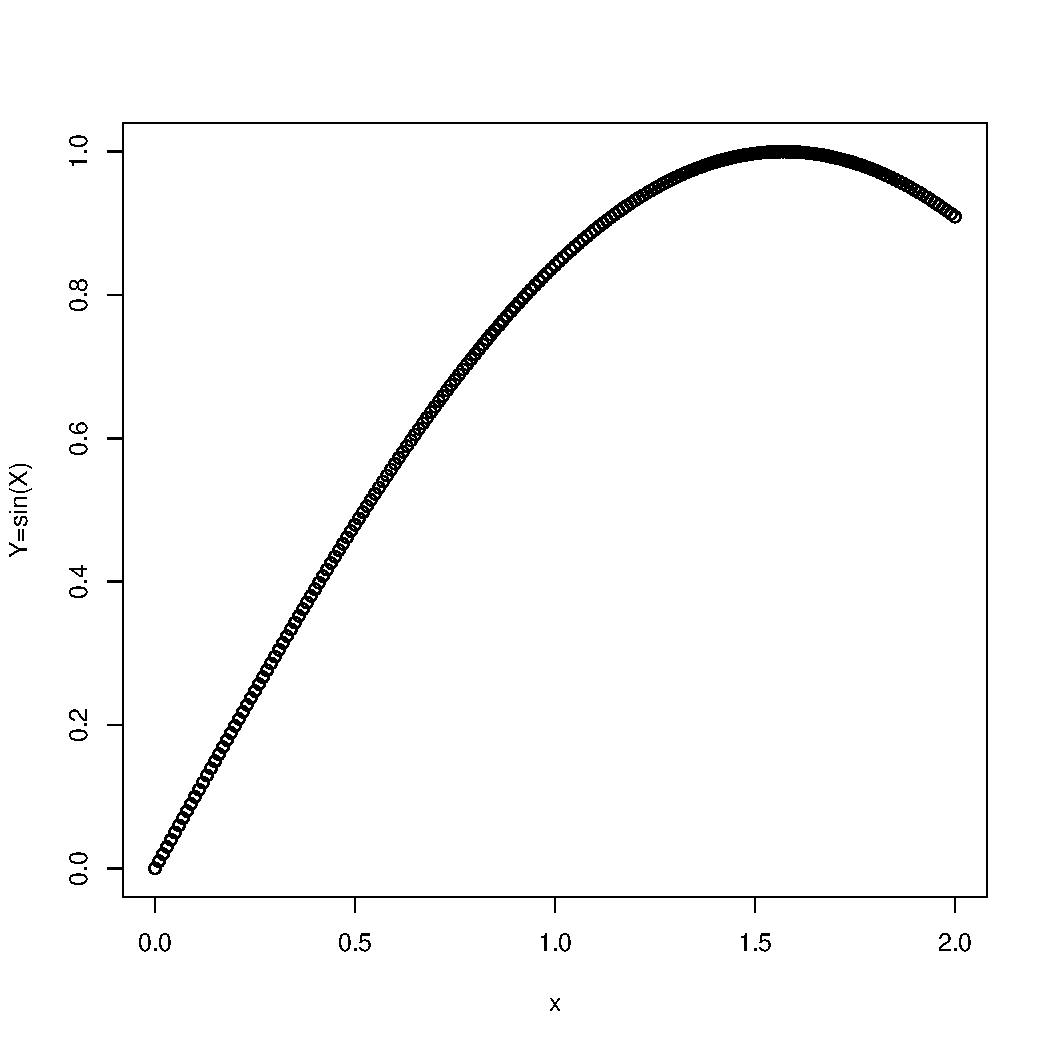
\includegraphics{hw1fig1redo.pdf}
\caption{A figure to show the relationship between $X$ and $Y$}
\end{figure}

\end{document}


